\documentclass[12pt,fleqn]{article}
\setlength{\parindent}{0pt}
\usepackage{graphicx}
\usepackage{cancel}
\usepackage{listings}
\usepackage[latin5]{inputenc}
\usepackage{color}
\setlength{\parskip}{8pt}
\setlength{\parsep}{0pt}
\setlength{\headsep}{0pt}
\setlength{\topskip}{0pt}
\setlength{\topmargin}{0pt}
\setlength{\topsep}{0pt}
\setlength{\partopsep}{0pt}
\setlength{\mathindent}{0cm}
\usepackage{latexsym}
\usepackage{amsfonts}
\usepackage{mathrsfs}
\usepackage{showkeys}
\renewcommand*\showkeyslabelformat[1]{(#1)}

\begin{document}
Ders 24

Green'in Teorisinin iki seklini gormustuk

\[ \oint_C \vec{F} \cdot \vec{T} ds = \int \int_R curl \ \vec{F} \ dA \]

\[ \oint_C \vec{F} \cdot \vec{n} \ ds = \int \int_R div \ \vec{F} \ dA \]


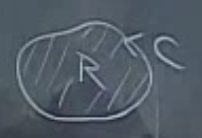
\includegraphics[height=2cm]{24_1.png}

Bu esitliklerin sag taraflarinin hesaplanabilir, anlamli olmasi icin vektor
alani $\vec{F}$'in $R$ icinde her yerde tanimli olmasi gerekir. Eger $R$
icinde tanimli olmayan tek bir nokta bile varsa, o zaman ustteki hesaplari
yapamayiz demektir.

Ornek 

\[ \vec{F} = \frac{ -y\hat{i} + +x\hat{j}}{x^2+y^2} \]

$\vec{F}$ orijinde tanimli degildir, eger alanin icinde orijin yok ise,
$curl \ \vec{F} = 0$, ama ayni orijini iceriyorsa, Green Teorisi
kullanilamaz, en azindan direk olarak kullanilamaz. 




\end{document}
